\documentclass[12pt]{article}
\usepackage{enumerate}
\usepackage{notes}
\usepackage{oxford}

\newcommand{\Ch}{\mathcal{C}_h}

\begin{document}
\title{Oxford M1 - Groups and Group Actions \footnotetext{\url{https://courses.maths.ox.ac.uk/node/5552}}}
\author{Dan Davison}
\maketitle

\section{Sheet 5: Homomorphisms. Conjugacy. Normal Subgroups.}

\begin{mdframed}
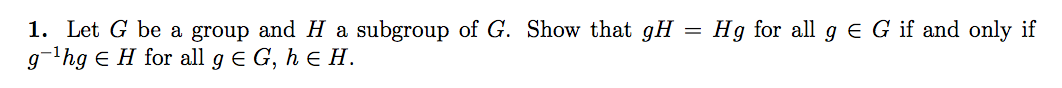
\includegraphics[width=400pt]{img/abstract-algebra-oxford-M1-5-1.png}
\end{mdframed}

\begin{claim*}
[Forwards implication]
  If $g^\1hg \in H$ for all $g \in G, h \in H$ then $gH = Hg$.
\end{claim*}

\begin{proof} We show that $Hg \subseteq gH$ and $gH \subseteq Hg$, for all $g \in G$.\\

Multiplying on the left by $g$ gives $hg \in gH$ for all $g \in G, h \in H$. Therefore $Hg \subseteq gH$ for all $g \in G$.
\end{proof}

\begin{mdframed}
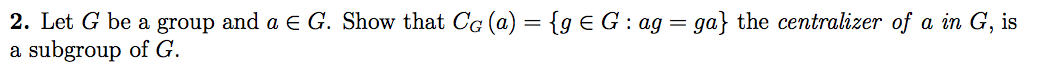
\includegraphics[width=400pt]{img/abstract-algebra-oxford-M1-5-2-1.png}
\end{mdframed}

\begin{mdframed}
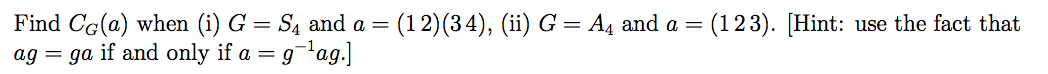
\includegraphics[width=400pt]{img/abstract-algebra-oxford-M1-5-2-2.png}
\end{mdframed}

\begin{mdframed}
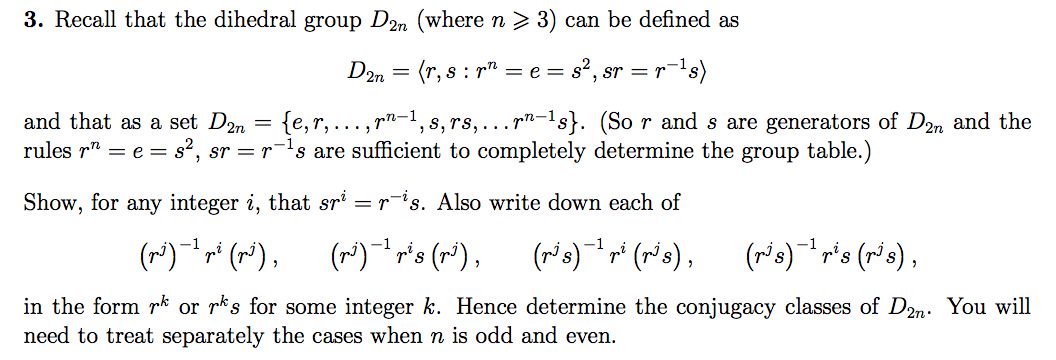
\includegraphics[width=400pt]{img/abstract-algebra-oxford-M1-5-3.png}
\end{mdframed}

\newpage
\section{Sheet 6: Quotient Groups. Isomorphism Theorem. Group Actions.}

\begin{mdframed}
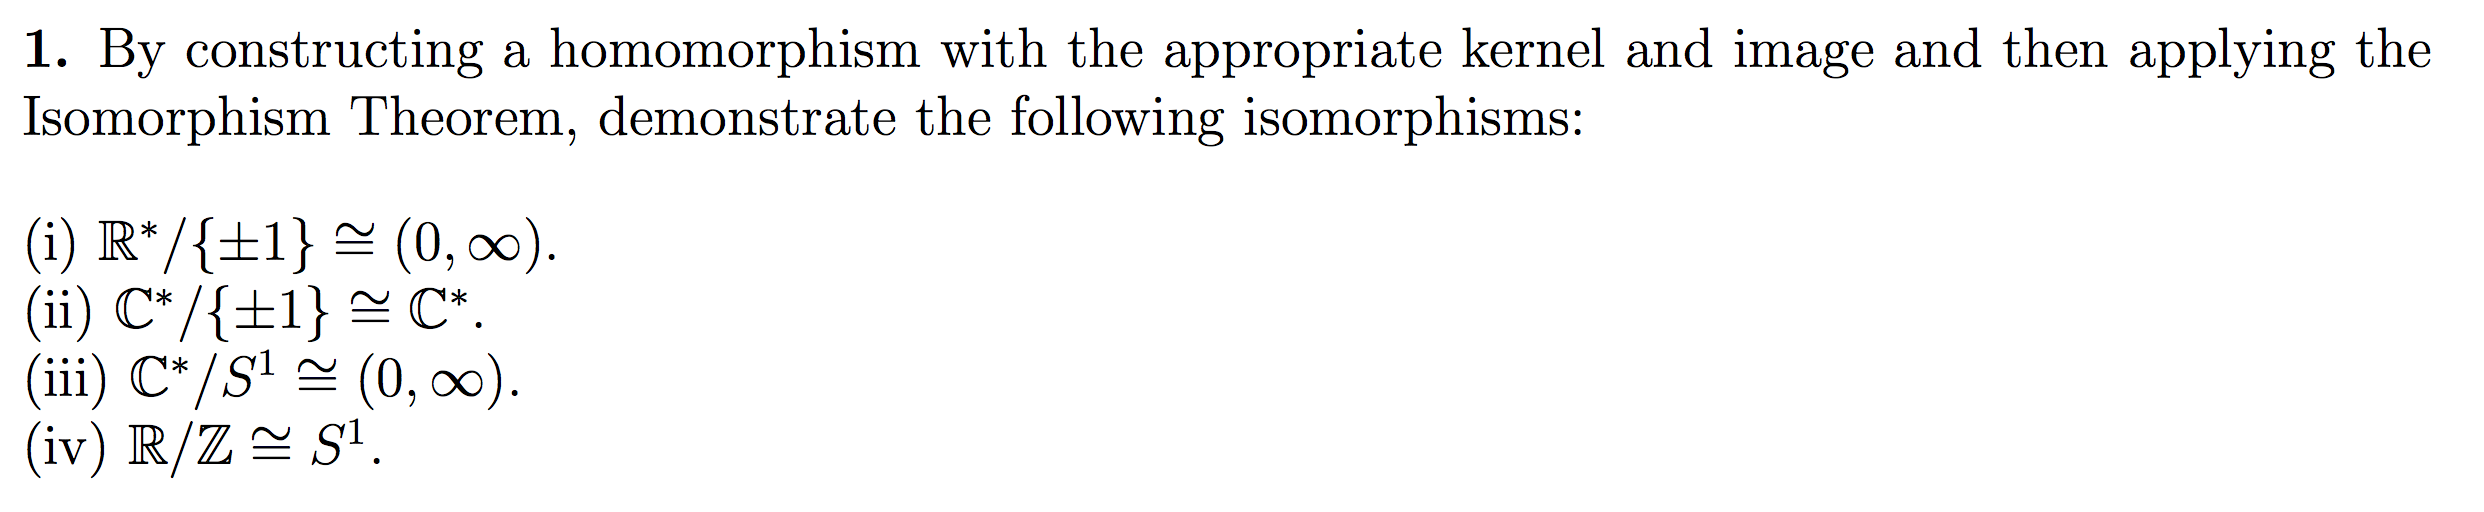
\includegraphics[width=400pt]{img/abstract-algebra-oxford-M1-6-1.png}
\end{mdframed}

\begin{theorem*}[First Isomorphism Theorem]~\\
  Let $\varphi:G_1 \to G_2$ and let $H$ be the kernel of $\varphi$. Then
  \begin{enumerate}
  \item $\Im \varphi \cong G/ \ker \varphi$
  \end{enumerate}
\end{theorem*}

\subsection*{(i): $\R^*/\{\pm 1\} \cong (0, \infty)$}

We have a group $G = \R^* = \R\setminus\{0\}$.

We have a subgroup $H = \{\pm 1\}$.

The group is abelian hence the subgroup is normal.

The set of cosets is $G/H = \{(0, \infty), (-\infty, 0)\}$.

Define the homomorphism $\varphi: G \to G/H$.

The image of $\varphi$ is the set of cosets $G/H$.

The kernel of $\varphi$ is $(0, \infty)$.

\end{document}
